\chapter*{Appendix}
\label{chapter:Appendix}
\pagestyle{Appendix}
\addcontentsline{toc}{chapter}{Appendix}

\section*{Appendix A: Vorauslegung}\label{Anh:programmcode}

\begin{figure}[H]
  \centering
  \includegraphics[width=\linewidth]{../../Code/radiator_leistung.pdf}
  \caption{Radiator Leistung nach Fläche und Temperatur}\label{fig:radiator_flaeche_leistung}
\end{figure}

\begin{figure}[H]
    \centering
    \begin{subfigure}{0.9\textwidth}
        \centering
        \includegraphics[width=\linewidth]{../../Code/pcm_mass.pdf}
        \caption{PCM Masse}\label{fig:pcm_mass}
    \end{subfigure}
    \vspace{1em}  % Optional vertical spacing
    \begin{subfigure}{0.9\textwidth}
        \centering
        \includegraphics[width=\linewidth]{../../Code/pcm_heat_capacity.pdf}
        \caption{PCM Wärmeaufnahme}\label{fig:pcm_heat}
    \end{subfigure}
    \caption{PCM Auslegung}\label{fig:pcm_mass_heat}
\end{figure}

\newpage

\begin{lstlisting}[language=C, caption={Vollständige \ac{pcm} \ac{udf} eicosane.c}, label={lst:udf_rest}]
//Modified UDF of the original source: https://akamcae.com/tutorials/phase-change-material-simulation-in-ansys-fluent/
#include "udf.h"
#include "mem.h"

//n-eicosane constant properties in solid phase
#define Ros_pcm 910.0
#define Cps_pcm 2132.4
#define Ks_pcm 0.4248

//n-eicosane constant properties in fluid phase
#define Rol_pcm 769.0
#define Cpl_pcm 2350.05
#define Kl_pcm 0.1505

//thermal expansion coefficient
#define TEC 0.0009

//solidus and liquidus temperatures of n-eicosane
#define Ts 309.0
#define Tl 311.0

//reference temperature for Boussinesq's approximation
#define Tr 310.0		//Fluent Tref must be equal to Tr

//density of PCM
DEFINE_PROPERTY(Ro_var_PCM,cell,thread)
{
	double Gama, Ro_pcm;
	#if !RP_HOST
		Gama=C_LIQF(cell,thread);
		Ro_pcm=(1-Gama)*Ros_pcm+Gama*Rol_pcm;
	#endif
	return Ro_pcm;
}

DEFINE_SPECIFIC_HEAT(Cp_var_PCM,T,Tref,h,yi)
{
	double Gama, Cp_pcm;
	#if !RP_HOST
		if (T<Ts) { Cp_pcm=Cps_pcm; } else if (T>=Ts&&T<=Tl)
		{
			Gama=(T-Ts)/(Tl-Ts);
			Cp_pcm=((1-Gama)*Ros_pcm*Cps_pcm+Gama*Rol_pcm*Cpl_pcm)/((1-Gama)*Ros_pcm+Gama*Rol_pcm);
		}
		else
		{
			Cp_pcm=Cpl_pcm;
		}
		*h=Cp_pcm*(T-Tref);
	#endif
	return Cp_pcm;
}

//thermal conductivity of n-eicosane
DEFINE_PROPERTY(K_var_PCM,cell,thread)
{
	double Gama, K_pcm;
	#if !RP_HOST
		Gama=C_LIQF(cell,thread);
		K_pcm=(1-Gama)*Ks_pcm+Gama*Kl_pcm;
	#endif
	return K_pcm;
}

//dynamic viscosity of PCM with fit
DEFINE_PROPERTY(Mu_var_PCM,cell,thread)
{
	double Temp,Mu_pcm;
	#if !RP_HOST
		Temp=C_T(cell,thread);
		Mu_pcm=(9*pow(10.,-4)*pow(Temp,2)-0.6529*Temp+119.94)*pow(10.,-3);
	#endif
	return Mu_pcm;
}

DEFINE_SOURCE(Boussinesq_momentum_source,cell,thread,dS,eqn)
{
	double Temp, source, acc;
	Temp=C_T(cell,thread);

	double t = CURRENT_TIME;

	if (t < 20)
		acc = 34.81;
	else if (t < 50)
		acc = 109.81;
	else if (t < 150)
		acc = 19.62;
	else
		acc = 9.81;

	source=-Rol_pcm*acc*TEC*(Temp-Tr); //negative for -Y down
	dS[eqn]=-Rol_pcm*acc*TEC; //negative for -Y down
	return source;
}
\end{lstlisting}

% \begin{lstlisting}[language=python, caption={setup.json}, label={lst:setup.json}]
% {
%     "devmode": 0,
%     "avionics_power": 40,
%     "target_temperature": 36.85,
%     "emittance": 0.91,
%     "absorptance": 0.15,
%     "solar_flux": 1000,
%     "trajectory_data_path": "blast.csv"
% }
% \end{lstlisting}

% \begin{lstlisting}[language=python, caption={results.json}, label={lst:results.json}]
% {
%     "hybrid_radiator_area": 0.0996163285294786,
%     "hybrid_radiator_power": 47.471224639710904,
%     "hybrid_capacity_sim": 188087.64535959047,
%     "hybrid_capacity_nu": 626817.5705502237,
%     "pcm_capacity": 48000.0,
%     "hybrid_H_sim": 0.013188203298524867,
%     "hybrid_m_sim": 1.6535028624398134,
%     "hybrid_H_nu": 0.03928567591747304,
%     "hybrid_m_nu": 4.255679378864365,
%     "normal_L_solution": 0.06748627883089094,
%     "normal_m_solution": 0.346609735620966
% }
% \end{lstlisting}

% \begin{lstlisting}[language=python, caption={main.py}, label={lst:main.py}]
% import subprocess

% subprocess.run(["python", "radiator.py"])
% subprocess.run(["python", "hybrid.py"])
% subprocess.run(["python", "pcm.py"])
% subprocess.run(["python", "pcmProperty.py"])
% subprocess.run(["python", "post.py"])
% \end{lstlisting}

% \begin{lstlisting}[language=python, caption={radiator.py}, label={lst:radiator.py}]
% # This Program calculates the steady-state equation for a grey body radiator

% import numpy as np
% import json
% from scipy.constants import Stefan_Boltzmann, pi
% import matplotlib.pyplot as plt
% import matplotlib as mpl



% # === configuration ===
% # load data from setup.json
% try:
%     with open("setup.json", "r", encoding="utf-8") as f:
%         data = json.load(f)
% except FileNotFoundError:
%     print("setup.json not found. Exiting.")
%     exit()
% except json.JSONDecodeError:
%     print("setup.json is empty of invalid. Exiting.")
%     exit()

% DEVELOPMENT_MODE = data["devmode"]
% avionics_power = data["avionics_power"] # W
% e = data["emittance"]
% a = data["absorptance"]
% solar_flux = data["solar_flux"] # W*m^-2
% target_temperature = data["target_temperature"]

% # Set global matplotlib style
% mpl.rcParams.update({
%     "figure.figsize": (4.9, 3.5),
%     "font.size": 11.0,
%     "font.family": "serif",
%     "font.serif": ["cmr10"],
%     "axes.titlesize": "medium",
%     "figure.titlesize": "medium",
%     "text.usetex": not DEVELOPMENT_MODE,
%     "text.latex.preamble": r"\usepackage{amsmath}\usepackage{amssymb}\usepackage[=v2]{siunitx}\usepackage[utf8]{inputenc}"
% })



% # === Equations ===
% rho_alu = 2700 # kg/m^3
% T_target = 273.15+target_temperature # target temperature

% # Define temperature in Celsius for plotting, and convert to Kelvin
% temp_C = np.linspace(0, 100, 100) # ^\circ C
% A = np.linspace(0.01*0.01, 0.3*0.3, 100) # Area [m$^2$]

% A_grid, T_C_grid = np.meshgrid(A, temp_C)
% T_K_grid = T_C_grid + 273.15  # Convert Celsius to Kelvin for calculation

% # Stefan-Boltzmann radiation formula
% phi_radiation = (A_grid * e * Stefan_Boltzmann * T_K_grid**4) # [W]



% # === Target result ===
% hybrid_radiator_area = (avionics_power) / ((e * Stefan_Boltzmann * T_target**4)-(solar_flux/2)*a) # [m^2] necessary radiator area to get rid of avionics- and solarheatflux
% hybrid_radiator_power = hybrid_radiator_area*e*Stefan_Boltzmann*T_target**4 # [W] total out-heatflux of radiator

% # Putting Data into result.json
% with open("result.json", "w", encoding="utf-8") as f:
%     json.dump({}, f, indent=4)  # clear result.json as this is the first write in the programm chain

% data = {
%     "hybrid_radiator_area": hybrid_radiator_area,
%     "hybrid_radiator_power": hybrid_radiator_power
% }

% with open("result.json", "w", encoding="utf-8") as f:
%     json.dump(data, f, indent=4)



% # === Plotting ===
% # Plot
% fig1 = plt.figure(figsize=(8, 6))
% contour = plt.contour(A_grid, T_C_grid, phi_radiation, levels=20, colors='black')
% #plt.colorbar(contour, label='W\"arme [W]')   # colorful contours
% plt.clabel(contour, inline=True, levels=contour.levels[::2], fontsize=10, fmt='%1.1f [W]') # levels makes every second contour have a label
% plt.xlabel(r"Fl\"{a}che [m$^2$]")
% plt.ylabel(r"Temperatur [^\circ C]")
% plt.grid(True)

% if DEVELOPMENT_MODE:
%     plt.title(r"Radiator W\"armestrahlung nach Fl\"{a}che und Temperatur")

% # Save it if not in dev mode
% if not DEVELOPMENT_MODE:
%     fig1.savefig("radiator_leistung.pdf", bbox_inches="tight")

% if DEVELOPMENT_MODE:
%     plt.show()
% \end{lstlisting}

\section*{Appendix B: Simulation}\label{Anh:simulation}

\begin{figure}[H]
    \centering

    \begin{subfigure}{\textwidth}
        \centering
        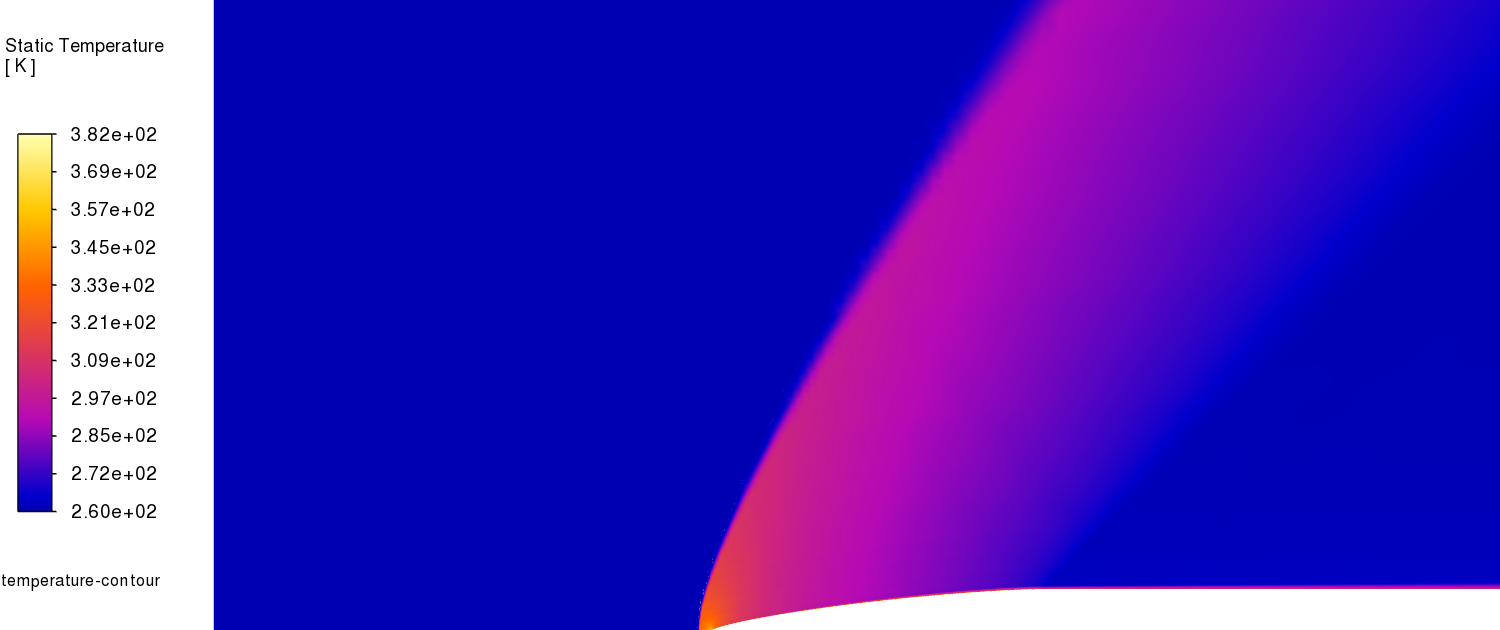
\includegraphics[height=0.23\textheight]{ansyspost/airflow/maxQminus10-temperature-contour.png}
        \caption{\ac{maxq} -\SI{10}{\second}}
        \label{fig:maxQminus10_temp_contour}
    \end{subfigure}

    \begin{subfigure}{\textwidth}
        \centering
        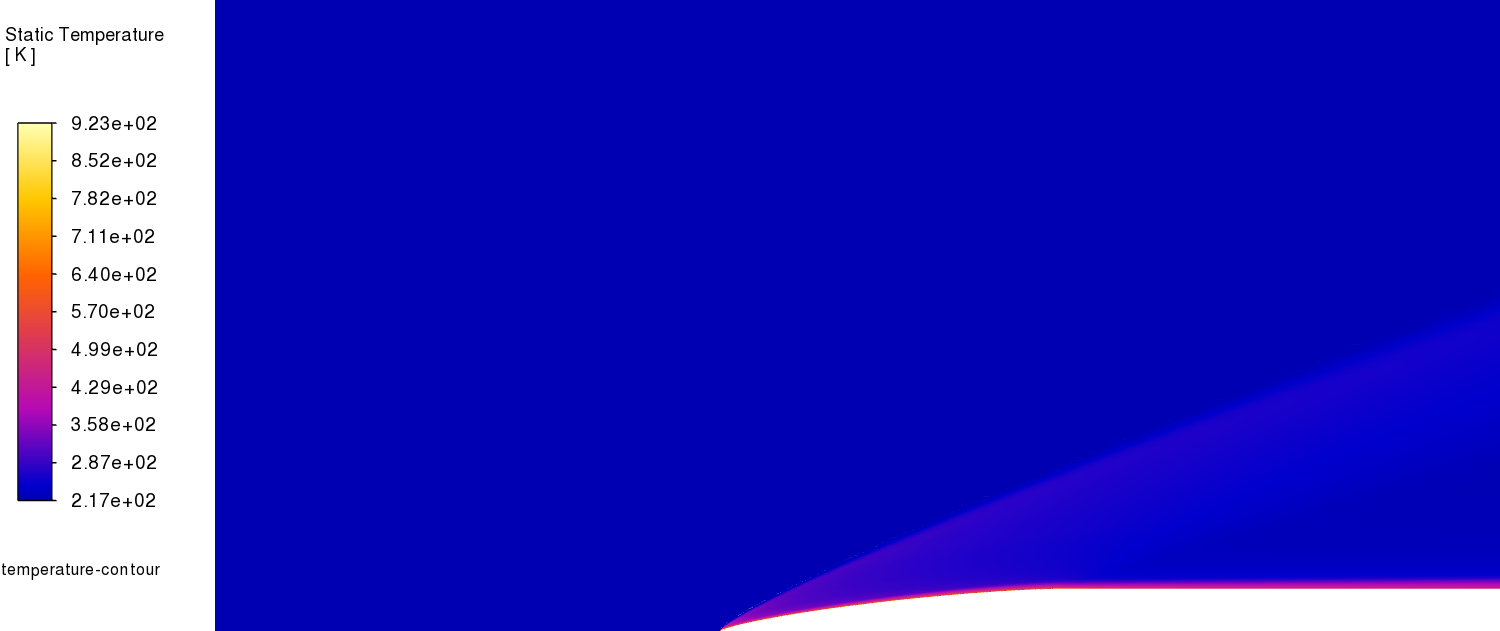
\includegraphics[height=0.23\textheight]{ansyspost/airflow/maxQplus10-temperature-contour.png}
        \caption{\ac{maxq} +\SI{10}{\second}}
        \label{fig:maxQplus10_temp_contour}
    \end{subfigure}

    \begin{subfigure}{\textwidth}
        \centering
        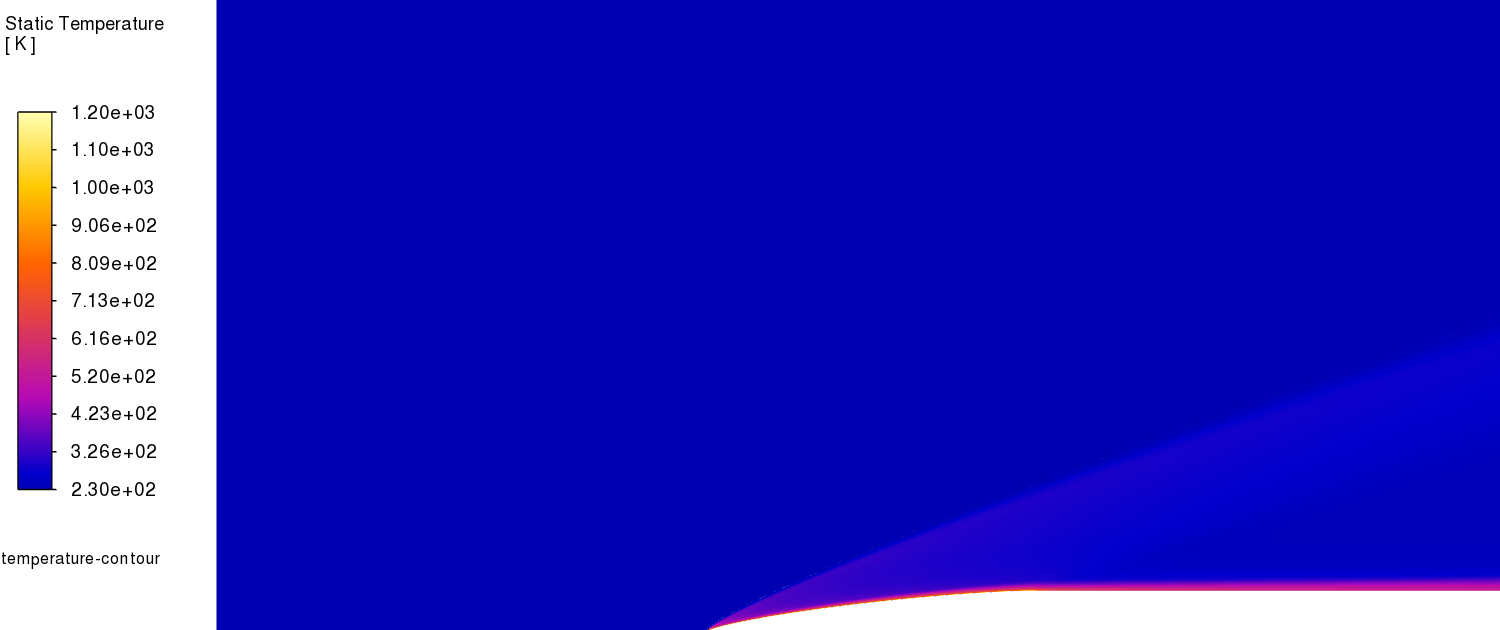
\includegraphics[height=0.23\textheight]{ansyspost/airflow/maxQplus20-temperature-contour.png}
        \caption{\ac{maxq} +\SI{20}{\second}}
        \label{fig:maxQplus20_temp_contour}
    \end{subfigure}

    \caption{Statische Temperaturkontur der Luft}
    \label{fig:airflow_temp_contour_continued}
\end{figure}

\begin{figure}[H]
    \centering

    \begin{subfigure}{\textwidth}
        \centering
        
\includegraphics[height=0.23\textheight]{ansyspost/airflow/maxQminus10-mach-contour.png}
        \caption{\ac{maxq} -\SI{10}{\second}}
        \label{fig:maxQminus10_mach_contour}
    \end{subfigure}

    \begin{subfigure}{\textwidth}
        \centering
        
\includegraphics[height=0.23\textheight]{ansyspost/airflow/maxQplus10-mach-contour.png}
        \caption{\ac{maxq} +\SI{10}{\second}}
        \label{fig:maxQplus10_mach_contour}
    \end{subfigure}

    \begin{subfigure}{\textwidth}
        \centering
        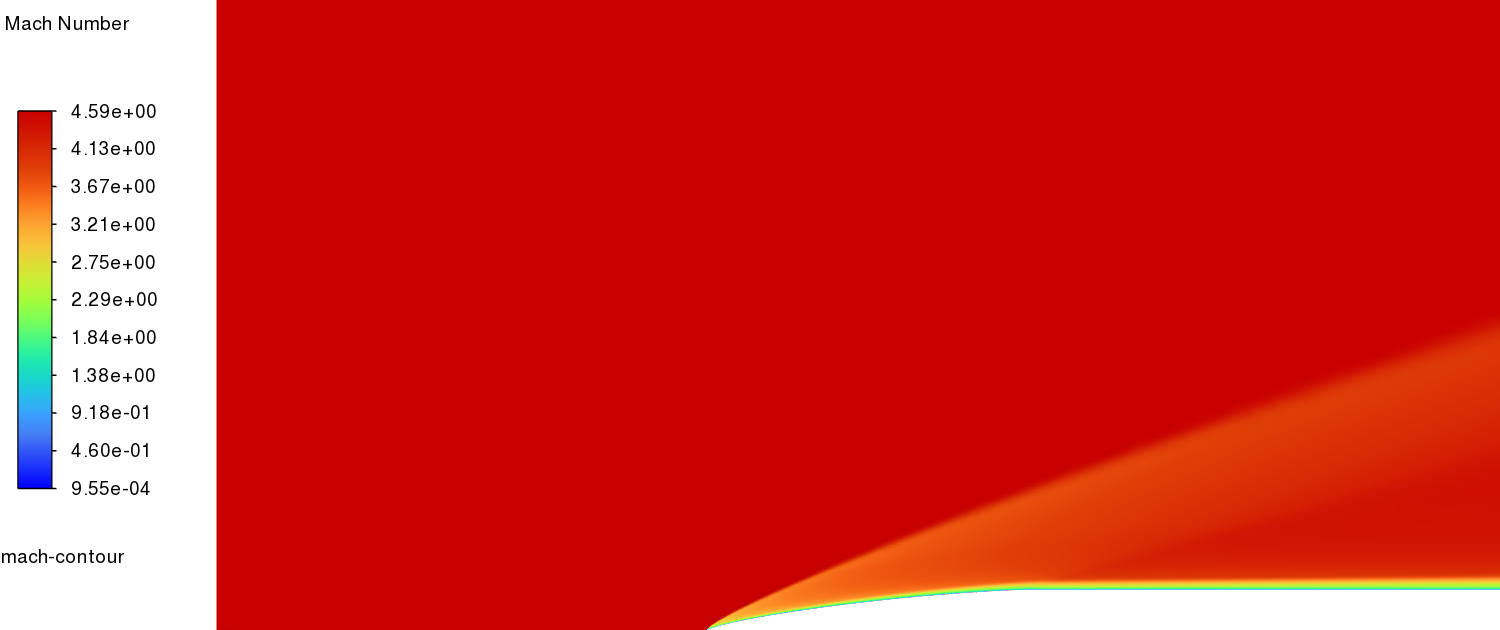
\includegraphics[height=0.23\textheight]{ansyspost/airflow/maxQplus20-mach-contour.png}
        \caption{\ac{maxq} +\SI{20}{\second}}
        \label{fig:maxQplus20_mach_contour}
    \end{subfigure}

    \caption{Machzahlkontur der Luft}
    \label{fig:airflow_mach_contour_continued}
\end{figure}

\begin{figure}[H]
    \centering

    \begin{subfigure}[t]{0.14\textwidth}
        \centering
        \raisebox{1\height}{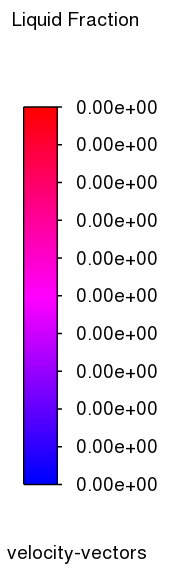
\includegraphics[height=0.2\textheight]{ansyspost/pcm/vector-legend.png}}
    \end{subfigure}%
    \hspace{2mm}% extra space between legend and first image
    \begin{subfigure}[t]{0.2\textwidth}
        \centering
        
\includegraphics[height=0.7\textheight]{ansyspost/pcm/velocity-vector-300.png}
        \caption{\SI{300}{\second}}\label{fig:velocity_vector_300}
    \end{subfigure}%
    \begin{subfigure}[t]{0.2\textwidth}
        \centering
        
\includegraphics[height=0.7\textheight]{ansyspost/pcm/velocity-vector-600.png}
        \caption{\SI{600}{\second}}\label{fig:velocity_vector_600}
    \end{subfigure}%
    \begin{subfigure}[t]{0.2\textwidth}
        \centering
        
\includegraphics[height=0.7\textheight]{ansyspost/pcm/velocity-vector-900.png}
        \caption{\SI{900}{\second}}\label{fig:velocity_vector_900}
    \end{subfigure}%
    \begin{subfigure}[t]{0.2\textwidth}
        \centering
        
\includegraphics[height=0.7\textheight]{ansyspost/pcm/velocity-vector-1200.png}
        \caption{\SI{1200}{\second}}\label{fig:velocity_vector_1200}
    \end{subfigure}
    \caption{Konturen der statischen Temperatur. Die Legende bezieht sich auf~\ref{fig:temperatur_1200}}\label{fig:pcm_static_temperature_kontur}
\end{figure}